\documentclass[12pt,a4paper,header]{abnt}

\usepackage[brazil]{babel}        
\usepackage[utf8]{inputenc} 

\usepackage{hyperref}
\usepackage{bookmark}
\usepackage{amsmath,amssymb,amsfonts,undertilde}
\usepackage{graphicx}
\usepackage{subfigure}
\usepackage{fancyhdr}

\usepackage{pdfpages} % Acrescentar pdf ficha bibliográfica

\usepackage[alf]{abntex2cite}	% Citações padrão ABNT


%%%%%%%%%%%%%%%%%%%%%%%%%%%
%Teoremas, definicoes, etc%
%%%%%%%%%%%%%%%%%%%%%%%%%%%

\newtheorem{thm}{Teorema}[chapter]
\newtheorem{cor}{Corolário}[chapter]
\newtheorem{lem}{Lema}[chapter]
\newtheorem{defi}{Definição}[chapter]
\newtheorem{exe}{Exemplo}[chapter]
\newtheorem{prop}{Proposição}[chapter]

\renewcommand{\ABNTchapterfont}{\bfseries}
\renewcommand{\ABNTsectionfont}{\bfseries}

\fancypagestyle{logouff}{%
	\renewcommand{\headrulewidth}{0pt}
	\fancyhead{}
	\fancyhead[R]{
\includegraphics[width=0.7\textwidth]{logoUFF.pdf}}% Your logo/image
  	\setlength{\headheight}{30pt} 
  	\setlength{\headsep}{2cm}
}

\begin{document}

%%%%%%%%%%%%%%%%%%%%%%%%%%%%%%
%colocar aqui o nome do aluno%
%%%%%%%%%%%%%%%%%%%%%%%%%%%%%%
\autor{João Pedro Abreu de Souza}


%%%%%%%%%%%%%%%%%%%%%%%%%%%%%%%%%%%%%
%colocar aqui o título da monografia%
%%%%%%%%%%%%%%%%%%%%%%%%%%%%%%%%%%%%%
\titulo{Título da Monografia}


%%%%%%%%%%%%%%%%%%%%%%%%%%%%%%%%%%%
%colocar aqui o nome do orientador%
%%%%%%%%%%%%%%%%%%%%%%%%%%%%%%%%%%%
\orientador{Prof. Dr. Nome do Orientador}  


%%%%%%%%%%%%%%%%%%%%%%%%%%%%%%%%%%%%%%%%%%%%%%%%%%%%
%colocar aqui o nome do co-orientador, caso exista%%
%se nao existir, comente a linha de codigo a seguir%
%ATENCAO: se nao houver co-orinetador também deve  %
%         ser comentada a linha 124, onde aparece  %
%         "Co-Orientador: & \ABNTcoorientadordata" %
%%%%%%%%%%%%%%%%%%%%%%%%%%%%%%%%%%%%%%%%%%%%%%%%%%%%
\coorientador{Prof. Dr. Nome do Co-orientador}


%%%%%%%%%%%%%%%%%%%%%%%%%%%%%%%%%%%%%%%%%%%%%%%%%%%
%colocar aqui a data da apresentacao da monografia%
%segue um exemplo								  %
%%%%%%%%%%%%%%%%%%%%%%%%%%%%%%%%%%%%%%%%%%%%%%%%%%%
\data{30 de fevereiro de 2013}

%%%%%%%%%%%%%%%%%%%%%%%%%%%
%nao mexer até a linha 170%
%%%%%%%%%%%%%%%%%%%%%%%%%%%

\comentario{Monografia apresentada para obtenção do grau de Bacharel em Estatística pela Universidade Federal Fluminense.}

\instituicao{Departamento de Estatística \par Instituto de Matemática e Estatística \par Universidade Federal Fluminense}

\local{Niterói - RJ, Brasil}

\capa

\vspace{10cm}



\begin{titlepage}

\thispagestyle{logouff}

\vspace{2cm}

\hspace{.2\textwidth} % posicionando a minipage
\begin{minipage}{.7\textwidth}

\begin{flushright}

{\large \bf \ABNTautordata} \\[3cm]

{\Large \bf \ABNTtitulodata}\\[3cm]

{\bf Trabalho de Conclusão de Curso}\\[1cm]

\end{flushright}

\begin{espacosimples}

\ABNTcomentariodata

\end{espacosimples}

\vspace{1cm}

\hfill 
\begin{tabular}{rl}
Orientador(a): & \ABNTorientadordata\\
%%%%%%%%%%%%%%%%%
% Comentar linha seguinte caso não haja co-orientador
Co-Orientador(a): & \ABNTcoorientadordata
\end{tabular}

\end{minipage}

\vspace{7cm}

\begin{center}

\ABNTlocaldata

\ABNTdatadata

\end{center}

\end{titlepage}


%folha de aprovacao com as assinaturas - Editar os membros da banca
\begin{folhadeaprovacao}

\thispagestyle{logouff}

\hspace{.2\textwidth} % posicionando a minipage
\begin{minipage}{.7\textwidth}

\begin{flushright}

{\large \bf \ABNTautordata}\\[1cm]

{\large \bf \ABNTtitulodata}\\[1cm]

\end{flushright}
Monografia de Projeto Final de Graduação sob o título \textit{``\ABNTtitulodata''},
defendida por \ABNTautordata~e aprovada em \ABNTdatadata, na cidade de Niterói,
no Estado do Rio de Janeiro, pela banca examinadora constituída pelos
professores:
\begin{flushright}

\begin{espacosimples}




%Folha de assinaturas
%%%%%%%%%%%%%%%%%%%%%%%%%%%%%%%%%%%%%%%%%
%Preencher os dados dos membros da banca%
%%%%%%%%%%%%%%%%%%%%%%%%%%%%%%%%%%%%%%%%%

\vspace{1.5cm}
\noindent\rule{10cm}{0.4pt}\\
{\bf Profa. Dra. Nome do Orientador}\\
Departamento de Estatística -- UFF\\

%se o trabalho não tiver co-orientator, comentar as 4 linhas que seguem
\vspace{1.5cm}
\noindent\rule{10cm}{0.4pt}\\
{\bf Prof. Dr. Nome do Co-Orientador}\\
Departamento de Estatística -- UFF\\

\vspace{1.5cm}
\noindent\rule{10cm}{0.4pt}\\
{\bf Prof. Me. Nome do 1o membro da banca}\\
Instituicao do 1º membro da banca\\


\vspace{1.5cm}
\noindent\rule{10cm}{0.4pt}\\
{\bf Profa. Ma. Nome do 2o membro da banca}\\
Instituicao do 2º membro da banca\\

\end{espacosimples}

\end{flushright}

\vspace{1.5cm}
\hfill Niterói, \ABNTdatadata

\end{minipage}

\end{folhadeaprovacao}


%%%%%%%%%%%%%%%%%%%%%%%%%%%%%%%%%%%%%%%%%%%%%%%%%%%%%%%%%%%%
% inclusão de ficha bibliográfica
% retire o símbolo de comentário e corrija o nome do arquivo
%%%%%%%%%%%%%%%%%%%%%%%%%%%%%%%%%%%%%%%%%%%%%%%%%%%%%%%%%%%%

%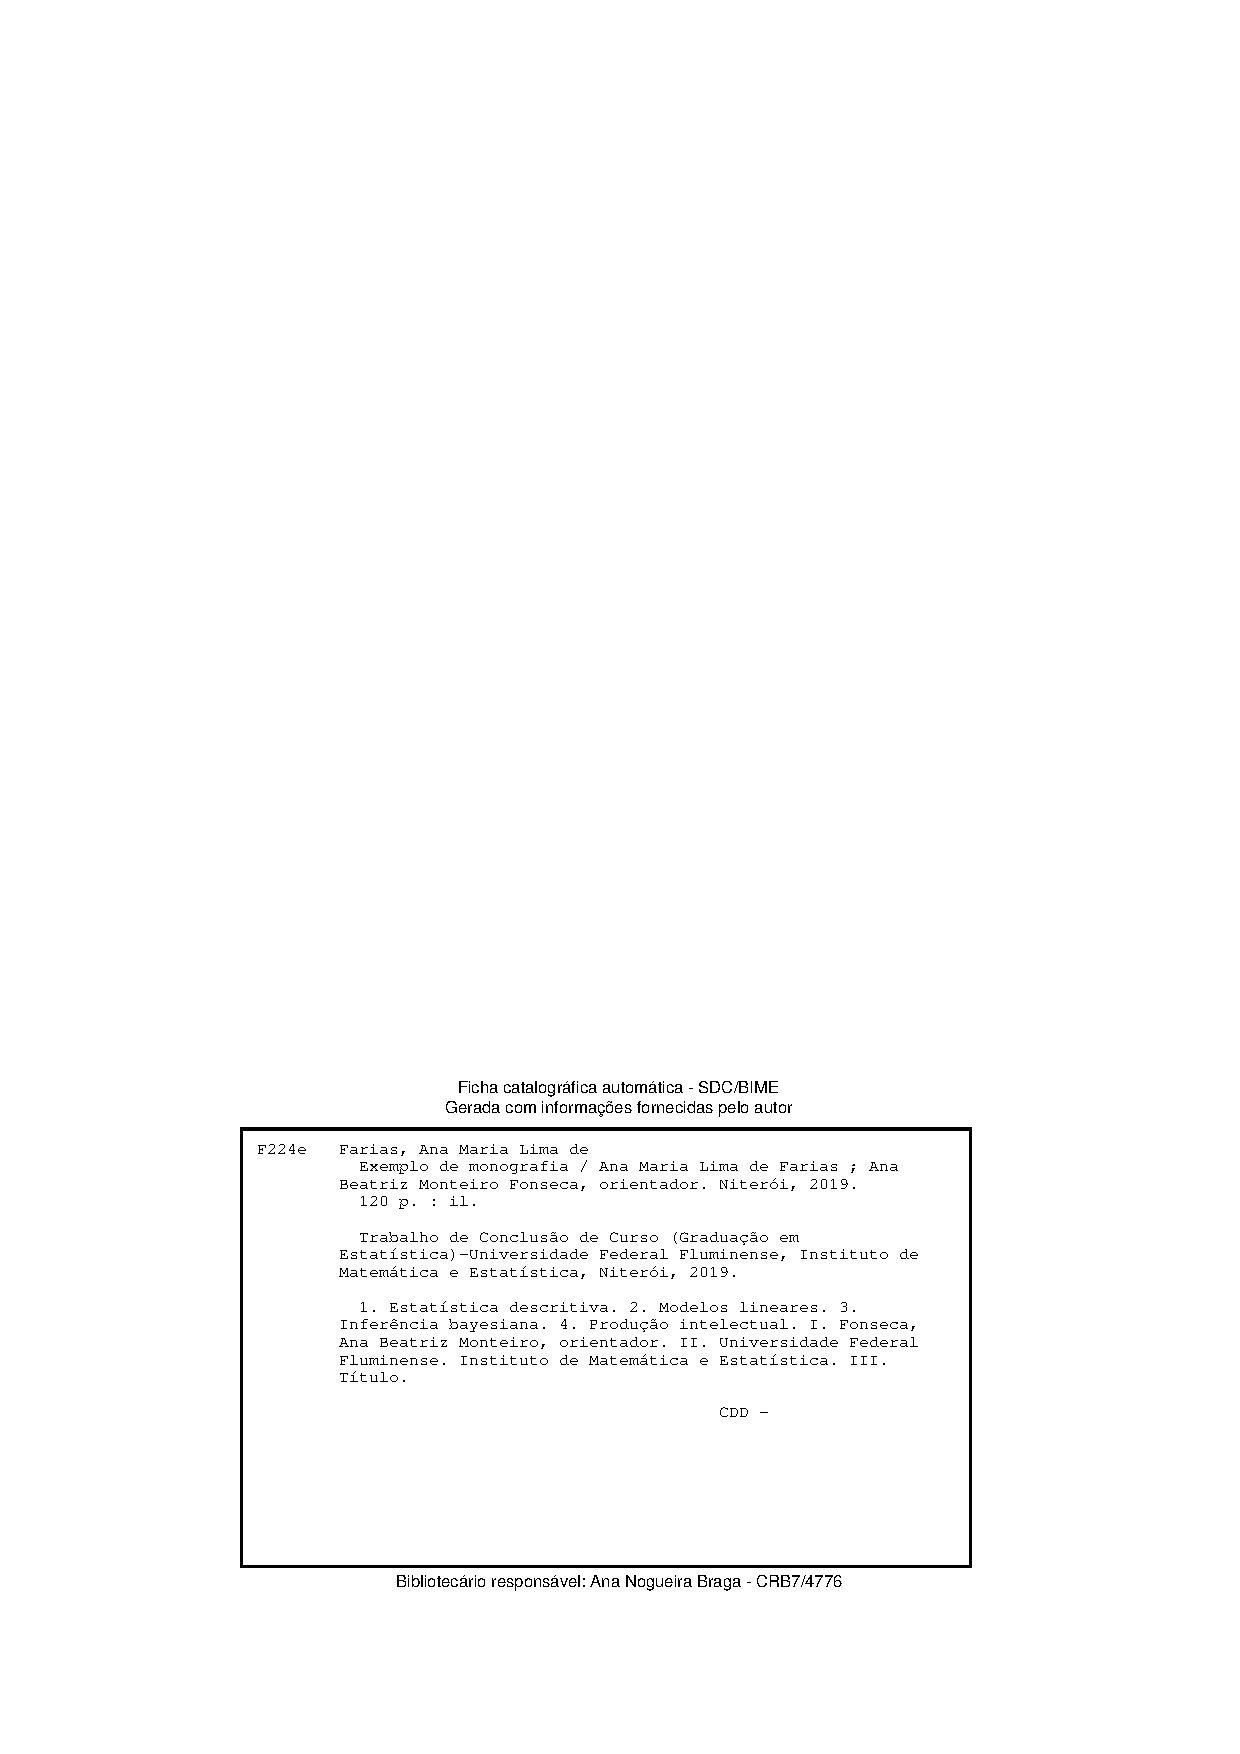
\includepdf[pages=-]{ficha.pdf}

%%%%%%%%%%%%%%%%%%%%%%%%%%%%%%%%%%%%%%%
%escreva aqui o resumo do seu trabalho%
%%%%%%%%%%%%%%%%%%%%%%%%%%%%%%%%%%%%%%%
\begin{resumo}
Aqui entra o resumo da monografia. Escreva o seu resumo na 3ª pessoa do singular, em um único parágrafo contendo entre 150 e 500 palavras. As palavras-chave devem entrar logo abaixo do resumo. Elas vêm em seguida de ``Palavras-chave:'', iniciadas por letras maiúscula e separadas por ponto. Veja um exemplo a seguir. Na ficha catalográfica só é permitida a inclusão de 4 palavras-chave; assim, escolha as 4 principais para o seu trabalho.



\vspace{1cm}
\noindent Palavras-chave: Estatística. Modelos lineares. Processo de Poisson. Estimador de máxima verossimilhança.



\end{resumo}



%%%%%%%%%%%%%%%%%%%%%%%%%%%%%%%%
%escreva aqui a sua dedicatória% (opcional)
%%%%%%%%%%%%%%%%%%%%%%%%%%%%%%%%
\chapter*{Dedicatória}
Aqui entra a sua dedicatória. 



%%%%%%%%%%%%%%%%%%%%%%%%%%%%%%%%%%
%escreva aqui seus agradecimentos% (opcional)
%%%%%%%%%%%%%%%%%%%%%%%%%%%%%%%%%%
\chapter*{Agradecimentos}
Aqui entram os agradecimentos. 



\tableofcontents{}
\listoffigures
\listoftables


%%%%%%%%%%%%%%%%%%%%%%%%%%%%%%%%%%%%%%%%%%%%
%Aqui começam os capítulo da sua monografia%
%%%%%%%%%%%%%%%%%%%%%%%%%%%%%%%%%%%%%%%%%%%%

\chapter{Introdução} \label{cap:introducao}


Escreva aqui o capítulo introdutório da sua monografia. 

\section{Motivação} \label{sec:motiv}
Contextualize o problema e apresente motivações para o desenvolvimento deste trabalho. Esse capítulo pode ou não ser separado em seções, faça como achar melhor. 



\section{Revisão Bibliográfica}
como visto no \ref{sec:motiv}
Se for interessante incluir uma revisão bibliográfica, ela pode entrar numa seção de introdução ou em um capítulo a parte, como você preferir.  


\section{Objetivos}
Independente se você optou por separar esse capítulo em seções ou não, é importante deixar bem claro e em destaque o objetivo do seu trabalho. Para isso, apresente os objetivos do seu trabalho ou em uma seção titulada ``Objetivos'' ou em seguida à palavra \textbf{\large Objetivos}, de preferência apresentada em negrito e com uma fonte maior. 

Para descrever os objetivos do seu trabalho use verbos no infinitivo. Se quiser pode dividir seus objetivos em gerais e específicos (ou principal e secundário). 


\section{Organização}
O último parágrafo desse capítulo deve apresentar a organização do seu trabalho. Em um único parágrafo, de forma breve e objetiva, descreva o que o leitor encontrará em cada capítulo que segue.





\chapter{Materiais e Métodos}

Apresente aqui os materiais e métodos usados na monografia. Este capítulo pode ser modificado de acordo com o interesse do aluno e do orientador. 

\section{Algumas Dicas}

\begin{itemize}

\item 
Separe o texto em seções para melhor organizar o trabalho. Use os comandos \verb|\section| e \verb|\subsection| para isso. 

\item 
Faça as referências usando os comandos 
\begin{center}
\verb|\citeauthor|, \verb|\citeyear|, \verb|\cite| e \verb|\citeonline|.
\end{center} O formato resultante do comando \verb|\citeonline| é o mais adequado para esse trabalho. Veja alguns exemplos:
\begin{itemize}

\item ``Para mais informações sobre esse assunto consulte o livro de \citeonline{larson} ou o de \citeonline{casella}''.

\item ``Em \citeyear{james} \citeauthor{james} publicou \ldots''

\item ``Uma estatística é qualquer transformação da amostra que não depende de parâmetros desconhecidos \cite{casella}''.

\end{itemize} 

\item Não use o comando \verb|\citep| para fazer referências. 

\item Mais informações sobre comandos do \LaTeX\ podem ser encontrados nas apostilas da professora \citeauthor{jessica_latex_basico} (\citeyear{jessica_latex_basico} e \citeyear{jessica_latex_intermediario}).

\end{itemize}

\section{Como apresentar Definições, Teoremas, \ldots}

As linhas 20-25 deste arquivo (.tex) definem comandos para que a numeração das definições, teoremas, etc sejam feitas de forma automática. Use os comandos a seguir para que isso aconteça. 

{\defi
Abra e feche as chaves e dentro delas coloque o comando \verb|\defi| seguido da definição. A numeração segue o seguinte padrão: primeiro o número do capítulo onde a definição aparece, em seguida um ponto e depois o número da definição dentro do capítulo.
}

{\thm
Abra e feche as chaves e dentro delas coloque o comando \verb|\thm| seguido do enunciado do teorema. A numeração segue o mesmo padrão descrito acima. 
}

{\prop
Abra e feche as chaves e dentro delas coloque o comando \verb|\prop| seguido do enunciado da proposição. A numeração segue o mesmo padrão descrito acima. 
}


{\exe
Abra e feche as chaves e dentro delas coloque o comando \verb|\exe| seguido do exemplo. A numeração segue o mesmo padrão descrito acima. 
}

{\exe
A segunda vez que você apresentar um exemplo a numeração será alterada. O mesmo vale para os teoremas, definições \ldots
}



\chapter{Análise dos Resultados}

Neste capítulo devem ser apresentados os resultados do seu trabalho, assim com as análises sobre eles. Aproveite para comentar, discutir e comparar os seus resultados com outros existentes na literatura. Separe esse capítulo em seções, como achar mais adequado. 

Para que as tabelas e figuras sejam incluídas corretamente nas listas de tabelas e figuras, que são criadas de forma automática no início do trabalho, use os comandos 
\begin{itemize}
\item \verb|\begin{table}| \ldots \verb|\end{table}| 
\item \verb|\begin{figure}| \ldots \verb|\end{figure}|
\end{itemize} 

Veja primeiro o exemplo de como incluir uma tabela. 

\begin{table}[h!]
\centering
\caption{Tabela exemplo} \label{fig:exemplo}
\begin{tabular}{cc}
\hline
Ano & Produção (1.000t)\\
\hline
1998 & 3.750\\
1999 & 2.007\\
2000 & 2.080\\
\hline
\end{tabular}
\end{table}

Agora veja como incluir uma figura. 
 
\begin{figure}[ht!]
\centering

\includegraphics[width=0.4\linewidth]{mascote.jpg}
\caption{Figura exemplo} \label{tab:exemplo}
\end{figure}

Use o comando \verb|ref| para fazer referências das tabelas e figuras ao longo do texto. Por exemplo, podemos nos referencias à Figura \ref{fig:exemplo} ou à Tabela \ref{tab:exemplo}.

O mesmo comando \verb|ref| pode ser usado para fazer referências a capítulos, seções, equações, \ldots Basta que tenha sido definido uma \verb|label| para cada um deles. Por exemplo, se quiser fazer uma referência ao capítulo de introdução primeiro cria-se um \textit{label} no início do capítulo, por exemplo, cria-se o \textit{label} ``cap:introducao'' usando o comando \verb|\label{cap:introducao}|, e depois digita-se o comando  
\verb|\ref{cap:introducao}| no local onde a referência será feita. Veja como: ``\ldots como comentado no Capítulo \ref{cap:introducao} \ldots''.



Por fim, se você usou o Programa R \cite{R} nas suas análises, não esqueça de citá-lo de forma correta, como foi feito aqui. 

\chapter{Conclusões}

Para finalizar seu trabalho faça o capítulo de conclusão. Neste capítulo deve ser feito um resumo do que foi feito e dos resultados encontrados. 





%%%%%%%%%%%%%%%%%%%%%%%%%%%%%%%%%%%%%%%%%%%%%%%%%%%%%%%%%%%%
%REFERENCIAS
%A bibliografia é feita automaticamente com o comando abaixo. 
%No arquivo referencias.bib devem ser incluídos todos os textos referenciados nesse trabalho.
%%%%%%%%%%%%%%%%%%%%%%%%%%%%%%%%%%%%%%%%%%%%
\bibliography{referencias}





%%%%%%%%%%%%%%%%%%%%%%%%
%%%INÍCIO DOS APENDICES%
%%%%%%%%%%%%%%%%%%%%%%%%
\apendice
\renewcommand\thechapter{\arabic{chapter}}

\chapter{Título do primeiro apêndice}

Cada apêndice é iniciado com o comando \verb|\chapter{}| e dentro das chaves colocamos o título do apêndice, assim como foi feito com os capítulos. 

Nos apêndices são incluídos textos elaborados pelo próprio autor. Dentro dos a\-pên\-di\-ces também podem ser feitas citações: ``No livro de \citeonline{ross_probability} \ldots''

\chapter{Título do segundo apêndice}
Dessa forma você pode incluir quantos apêndices quiser. Se não quiser incluir apêndice algum basta apagar as linhas de código referentes a eles no arquivo .tex. 





%%%%%%%%%%%%%%%%%%%%%%%%
%%%INÍCIO DOS APENDICES%
%%%%%%%%%%%%%%%%%%%%%%%%


%Os anexos devem ser intorduzidos ao final do trabalho, depois das referências
\anexo
\renewcommand\thechapter{\arabic{chapter}}

\chapter{Título do primeiro anexo}


Cada anexo é iniciado com o comando \verb|\chapter{}| e dentro das chaves colocamos o título do apêndice, assim como foi feito com os capítulos. 


Nos anexos são apresentados materiais desenvolvidos por outras pessoas. Dentro dos anexos também podem ser feitas citações, por exemplo, ``Veja em \citeonline{ross_simulation} como \ldots''



\chapter{Título do segundo anexo}
Dessa forma você pode incluir quantos anexos quiser. Se não quiser incluir anexo algum basta apagar as linhas de código referentes a eles no arquivo .tex. 



\end{document}
